\chapter{Methodology}
\label{chap:methodology}

In order to address the research questions, we need to develop a proof of concept system that is able to investigate and utilize the concepts in question. It was decided that a to-do list application would be a good candidate for investigating these concepts. A calendar would also be suitable, but a to-do list application was chosen over this because of simplicity.

The most natural choice of platform is mobile devices. This is because we are creating a context-aware application, and contextual information are more easily available on such devices because of the integrated sensors. On such devices it is easy to access information such as user activity, time and location. The Android Operating System was chosen for development, mostly because it holds the biggest market share, but also because an Android device was easily available for development.



\section{User group}
For the recommender to be able to differ between user tasks, these tasks needs to be assigned different types and be categorized. However, categorizing typical and everyday tasks will require a lot of effort. In order to reduce the amount of work needed for this, it was decided that the scope should be narrowed down by selecting a specific user group. Students were selected for this, and more specifically students in an educational environment. This is both because the tasks of such a specific user groups can be much easier categorized, but also because access to the user group is easily available in this case.

Although students were selected as the target user group, typical educational tasks can vary greatly between undergraduate and postgraduate students. This is also dependent on what semester the student in question is currently in. A bachelor student might have very different tasks than a master student doing his/hers master thesis. A small questionnaire was made to determine if we needed to differ between these two types of students. The results of the questionnaire, see Section~\ref{sec:studenttasks}, reported small differences between the tasks of the different types of students. It was thereby decided that the tasks should be categorized for all students.



\section{Application}

\subsection{General application design}
By choosing to create a todo-list application the user should be able to perform actions that are normal for such applications. These actions include creating and storing tasks, as well editing and deleting them. The tasks should also be possible to arrange into lists. The application in this study is developed in a way that supports all these aspects. When a todo-item or task is created, a date will be attached to that particular task, thereby organizing the tasks with similar dates into lists.

We would also need a schema for storing context information, as well as a recommender that will process the stored contexts and provide recomendations. A conceptual model of the application is shown in Figure~\ref{fig:conceptualmodel}. The lines pointing towards the recommender represents its input, whereas the line pointing outward is the actual recommendation. The input for the recommender consists of three parts:
\begin{itemize}
	\item The tasks that the user needs to do (planned tasks).
	\item The tasks that the user has previously done (task history).
	\item The contexts of related to the previously done tasks (context history).
	\item The users current context.
\end{itemize}
By taking all these components into account, the recommender will be able process the information and suggest a task for the user.

\begin{figure}[tbp]
  \centering
  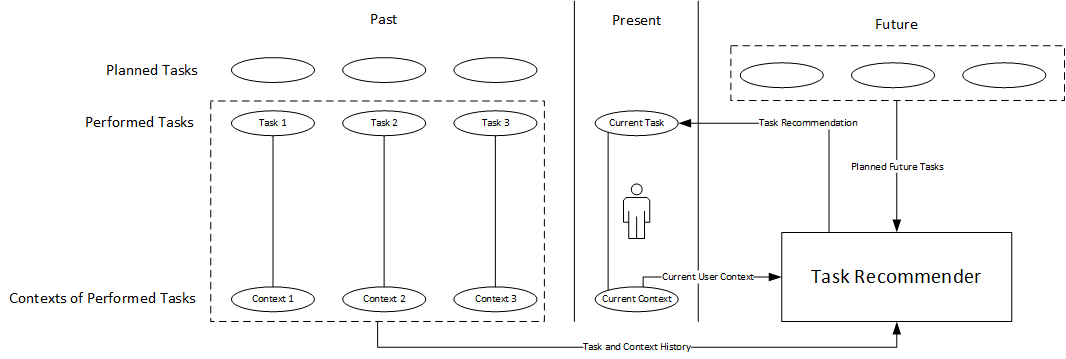
\includegraphics[width=\textwidth]{figures/ConceptualDiagram.png}
  \caption[Conceptual model]{Conceptual model of the application.}
  \label{fig:conceptualmodel}
\end{figure}


\subsection{Context acquisition}
By storing contextual information about how tasks are performed, the recommender will be able to not only provide recommendations based on current and planned contexts, but also take into account in what contexts tasks have been done previously. A certain task may work well in one context and poorly in another. However, before designing the overall schema of context representation, decisions on what contexts to actually use and collect needs to be made. In a mobile device there are typically many types of contexts that can be potentially collected. These are:\ldots reference do context types + figure \ldots

The actual contexts collected in the app are:
\begin{itemize}
	\item \emph{Location:} Both the planned location of the task as well as the actual location of where the task is performed is stored.
	\item \emph{Activity:} 
	\item \emph{Time:} Each task is given timestamps both when they are started and ended. By doing this it is possible for the recommender to separate tasks that are done at specific times of the day, week or even month. Time spent doing a task is also tracked, as this may differ from the difference between the start and end times (users may pause doing a task).
\end{itemize}


\subsection{Context storage}
Describe how the contexts are stored in the database... representation.


\subsection{Recommender}

When creating the recommender-part of the application, several decisions needed to be made. First of all, we needed to decide what kind of recommendations to make. There where many possible ways to do this:
\begin{itemize}
	\item Location proximity recommendations.
  \item Recommendations based on time of day.
  \item Recommendations based on time spent on previous tasks.
  \item Recommend tasks with fixed starting times.
  \item Recommend tasks based on the shortest traveling distance between tasks.
  \item Recommendations based on regularity of task occurrences.
  \item Combinations of the above.
\end{itemize}


After deciding what to recommend, the underlying logic also needs to be decided. A recommender will need some form of logic for comparison, so that it can know that it should recommend one task over another. Such logic already exist in some systems. We have seen Netflix recommending movies and Amazon recommending books. It is necessary to analyze these systems for potentially reusable recommendation algorithms:

\subsubsection{Neural networks}
Neural networks describes the process in which the computer\ldots

\subsubsection{Probability calculations}
The second approach is to use probability calculations to perform the recommendations. This is the approach that was decided to be used in this project. 

Unfinished \ldots
